
\lstinputlisting[language=bash,basicstyle=\small]{python_codes/fieldstone_108/keywords}

\begin{center}
Code at \url{https://github.com/cedrict/fieldstone/tree/master/python_codes/fieldstone_108}
\end{center}

\par\noindent\rule{\textwidth}{0.4pt}

{\sl This stone was developed in collaboration with Paul Pitard.} 
\index{contributors}{P. Pitard}

\par\noindent\rule{\textwidth}{0.4pt}

%%%%%%%%%%%%%%%%%%%%%%%%%%%%%%%%%%%%%%%%%%%%%%%%%%%%%%%%%%%%%%%%%%%%%%%%%%%%%%%%%%%%%%%%%%%%%%%%%%%%

The article by Clark \etal (2005) \cite{clbr05} about "Dynamic topography produced by lower crustal flow against rheological strength heterogeneities bordering the Tibetan Plateau" is rather popular and has been cited over 300 times. It uses an analytical model to compute the 
dynamic pressure generated by a flow around an obstacle (the Sichuan Basin) which is then used as the driving load for the flexure equation in 
order to compute a vertical deflection. In what follows we go through their derivations first and then proceed to replicate their results.  

We assume that the lower crust is ductile and flows in a flat channel. A single obstacle is present in the middle of the domain corresponding to a rigid block or sub-regional crustal fragment modelled as a cylinder with its axis perpendicular to the direction of flow.
Its viscosity is taken to be infinite to make it rigid. 
We prescribe a unidirectional far-field flow U within the channel (far from the obstacle) 
and examine the effect of an impermeable rigid obstacle. 

\begin{center}
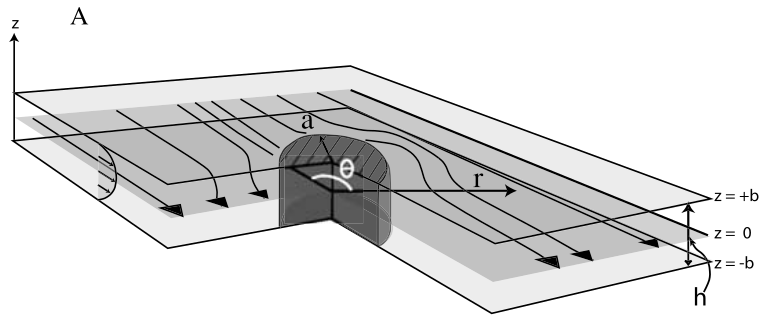
\includegraphics[width=10cm]{python_codes/fieldstone_108/images/clbr05a}\\
{\captionfont 
Taken from Clark \etal (2005). The center of the cylindrical coordinates axis system is in the middle of the cylinder.  
The far field velocity is aligned with the $x$-axis.}
\end{center}

The flow is characterised by no-slip boundary conditions on the top and bottom of the channel ($z=\pm b$) and flow symmetry produces parabolic channel flow $\vec\upnu$ :
\begin{equation}
\vec\upnu = -\frac{b^2}{2\eta} \vec\nabla P \left( 1 - \frac{z^2}{b^2} \right)
\end{equation}
where $2b$ is the height of the channel. The obstacle has a radius $a$. We can compute the depth-averaged flow:
\begin{equation}
\langle \vec\upnu \rangle = \frac{1}{2b} \int_{-b}^{+b} \vec\upnu \; dz 
=-\frac{b^2}{2\eta} \vec\nabla P \frac{1}{2b} 
\int_{-b}^{+b}   \left( 1 - \frac{z^2}{b^2} \right) dz
= -\frac{b^2}{2\eta} \vec\nabla P \frac{1}{2b} 
\left( 2b - \frac{1}{3b^2} 2b^3 \right)
= - \frac{b^2}{3\eta} \vec\nabla P 
= -\kappa \vec\nabla P
\label{eq:velo_para}
\end{equation}
where $\kappa$ is the effective permeability of the lower crust. 
Note that this is a Darcy-type flow equation.

No-slip boundary conditions are applied on the cylinder obstacle.
The appropriate solution for a 2D potential flow around a circle/cylinder is given by\footnote{\url{https://en.wikipedia.org/wiki/Potential_flow_around_a_circular_cylinder}}
\begin{eqnarray}
\langle\upnu_x(r,\theta)\rangle &=& U \left(1 -\frac{a^2}{r^2} \right) \cos \theta \label{eq:velo_para2}\\
\langle\upnu_y(r,\theta)\rangle &=& -U \left(1 +\frac{a^2}{r^2} \right) \sin \theta \label{eq:velo_para3}
\end{eqnarray}
where $U$ is the is the scalar value of the vertically averaged far-field flow, and the $\langle \cdot \rangle$
brackets indicate that these are vertically averaged fields.
\footnote{
If $\upnu = \upnu_0 (1-z^2/b^2)$ then 
$U=\frac{1}{2b} \int_{-b}^{+b} \upnu \; dz = 2\upnu_0/3$}
We of course find that when $r\rightarrow a$ then the velocity is zero 
(no-slip boundary conditions on the obstacle) and when $r\rightarrow \infty$ then the velocity tends to 
$(U \cos\theta, -U \sin\theta)$ as expected since $\theta$ is the angle made with the direction of far-field flow. 

The corresponding pressure field (excluding lithostatic pressure) is: 
\[
p(r,\theta) = -\frac{1}{\kappa} U \left( r  + \frac{a^2}{r}  \right)\cos \theta
\]
since it is trivial to verify that inserting this expression in Eq.~\eqref{eq:velo_para} yields the velocity components of Eqs.~\eqref{eq:velo_para2} and \eqref{eq:velo_para3} (remember that in polar coordinates the gradients operator is $\vec\nabla=(\partial_r , \frac{1}{r} \partial_\theta)$.

We find that the pressure field is only defined in the fluid, i.e. $r\geq a$ and that it depends on $\theta$ on the surface of the cylinder. Far from the cylinder this expression is a bit more problematic as it grows with $r$. We then split the pressure field as follows:
\[
p(r,\theta) = 
-\frac{1}{\kappa} U r  \cos \theta
 -\frac{U a^2 }{\kappa r}  \cos \theta
\]
Clark \etal (2005) attribute the first one to the background (far-field) Darcy-type flow ( $U \sim - \kappa p/r$) and the second to a local pressure field developed
due to flow being diverted around the rigid obstacle. They 
then proceed to discard the first and call the second the dynamic pressure $p_{dyn}$ which they use to drive a flexure equation. 
\[
p_{dyn}(r,\theta) = -\frac{U a^2 }{\kappa r}  \cos \theta
\]
The following figure shows the pressure field around the obstacle.
We find that the pressure is null on a direction perpendicular to the flow direction passing through the center of the obstacle ($\theta=\pi/2$) and its maximum positive and negative amplitude is reached on the line given by $\theta=0$.
\begin{center}
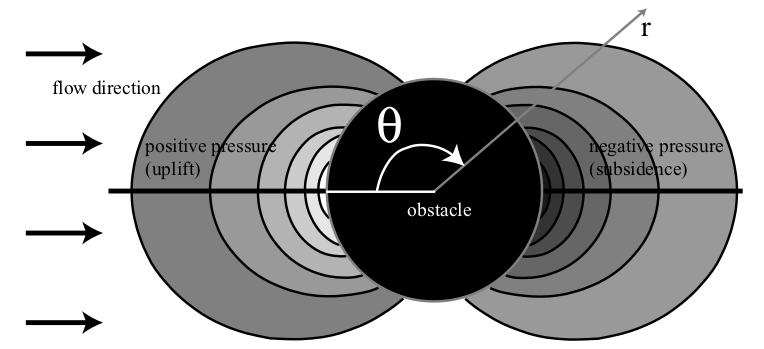
\includegraphics[width=7cm]{python_codes/fieldstone_108/images/clbr05b}\\
{\captionfont 
Taken from Clark \etal (2005). }
\end{center}

Under many simplifying approximations (See Section~3.9 of Turcotte \& Schubert book \cite{tusc}), 
the simplest time-independent flexure equation is
\[
D \frac{d^4w(x)}{dx^4} + P \frac{d^2w(x)}{dx^2} + (\rho_m-\rho_c)g w(x) = q(x)
\]
where $w(x)$ is the plate deflection (\si{m}), 
\[
D=\frac{E t^3}{12(1-\nu^2)}
\]
is the flexural rigidity, with $t$ the thickness of the plate (\si{m}), 
$E$ is Young's modulus, $\nu$ is the Poisson ratio, 
$P$ is a horizontal force per unit length (\si{\kg\per\square\metre\square\sec}),  
$q$ is the load (\si{\pascal}), 
$\rho_{lc}$ is the lower crust density and $\rho_{uc}$ is the density of the upper crust (\si{\kg\per\cubic\metre}).
This is a 4th-order Ordinary Differential Equation. 
In order to solve it, we will need 4 boundary conditions.

In the book the problem at hand is such that $t$ is the real thickness of the bending plate. 
In geophysics this quantity is replaced by the so-called Effective Elastic Thickness $T\!e$.
To quote Burov \& Diament (1995): ``The physical meaning and significance of the effective elastic thickness
for continents are still enigmatic, because for continental lithosphere estimates of Te bear little 
relation to specific geological or physical boundaries.'' 
See also Tesauro \etal (2012) \cite{teak12} for values of the effective elastic thickness of the continental lithosphere
on Earth.

The approach in Clark \etal is rather peculiar because they do not really address the question of the thickness
of the upper crust, although they draw it containing a viscous part and an elastic part:
\begin{center}
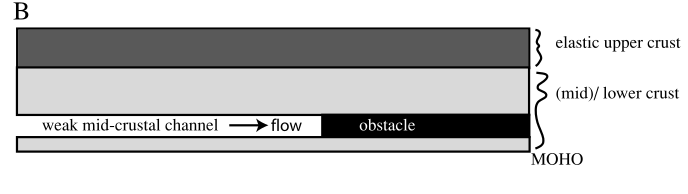
\includegraphics[width=7cm]{python_codes/fieldstone_108/images/clbr05d1}
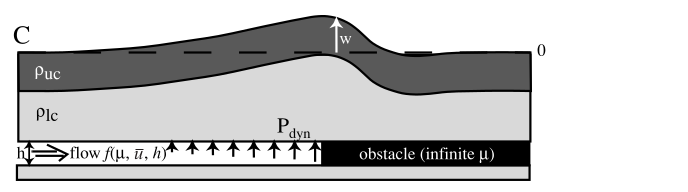
\includegraphics[width=7cm]{python_codes/fieldstone_108/images/clbr05d2}\\
{\captionfont  Taken from Clark \etal (2005). }
\end{center}
Instead the only upper crust property that is needed in the equation above is the effective elastic thickness. 



Clark \etal (2005) neglect the $P$ term, i.e. horizontal forces so that the equation becomes:
\[
D \frac{d^4w(x)}{dx^4} + \delta\!\rho \; g w(x) = q(x)
\]
where $\delta\rho$ is the density difference between the two layers (more on this later). 
They then assume that the dynamic pressure calculated above is the sole source of load on this elastic plate and then obtain 
\[
D \frac{d^4w(x)}{dx^4} + \delta\!\rho \; g w(x) = p_{dyn}(x)
\]
which is their Eq.~(10). Note that in fact $x$ should be understood as the coordinate $r$. Because $p_{dyn}$ depends on $\theta$ they can compute the deflection on any 1D line passing through the center of the obstacle. 

Solving this equation is rather trivial (see \stone~105) BUT we are missing the following things from their paper:
\begin{itemize}
\item boundary conditions on flexure equation. If domain is (very) large, we can assume standard ones. 
\item $\delta \rho$ value
\item they provide values for the effective elastic thickness $T\!e$ ($t$ in the equations above) but fail to report $E$ and $\nu$ so I cannot compute $D$. They however refer to Burov \& Diament \cite{budi95} and we find in there $E=6.5-8\cdot 10^{10}\si{\newton\per\square\meter}$ and $\nu=0.25$.
Taking $E=7\cdot 10^{10}$ yields $D = 6.222\cdot 10^9 T\!e^3$ 
\item the size of the domain (!)
\end{itemize}
The unescapable conclusion is that the paper is not replicable. Let us however make an attempt. 
We fix $\nu=0.25$ and $E=70\cdot10^{9}~\si{\pascal}$. We Take a ridiculously large domain
of 20,000~\si{\km} so as to avoid any interference of the boundaries on the results. 
Boundary conditions are $w=0$ and $w'=0$ on the left and right boundaries. 
Turning now to $\delta \rho$ one must recall that in \stone~105 it is $\rho_m-\rho_c$ with a load being prescribed atop the crust.
In our case the load is prescribed at the bottom of the crustal layer so the air above is the 'mantle layer' of \stone~105, so that 
$\delta\rho=\rho_{uc}-\rho_{air}=\rho_{uc}$ and we take $\rho_{uc}=2850~\si{\kg\per\cubic\meter}$. 
Gravity is set to $g=9.81~\si{\metre\per\square\second}$.

The code is not even 100 lines long. It solves the flexure equation, see \stone~105. The load is zero below the 
obstacle which is placed in the middle of the domain and equal to $p_{dyn}$ outside of it. 
We then run the same models as Clark \etal (2005)
and hope to reproduce the results of their Fig.~4 shown here under:

\begin{center}
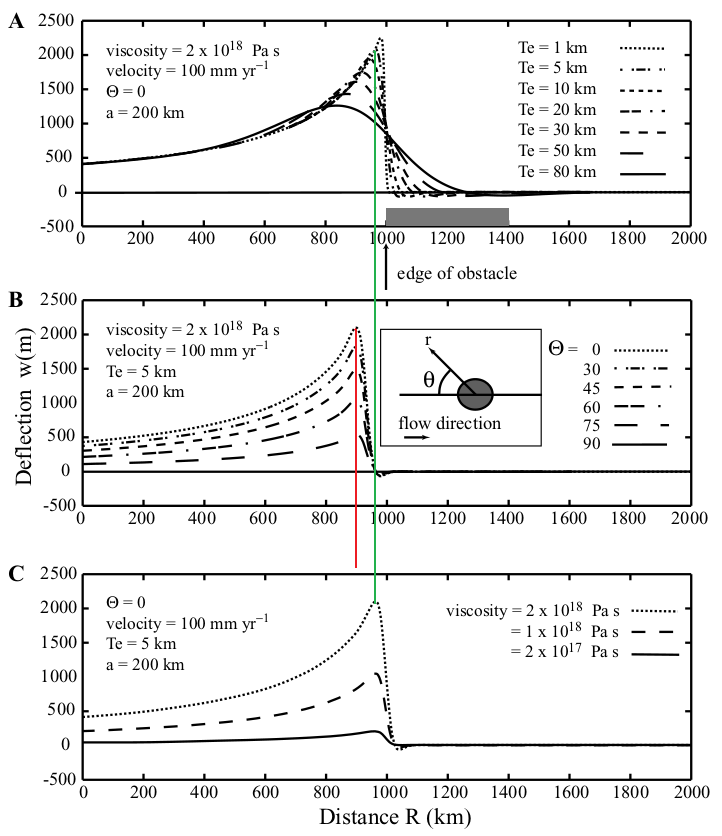
\includegraphics[width=12cm]{python_codes/fieldstone_108/images/clbr05c}\\
{\captionfont Taken from Clark \etal (2005). Note that all three 
subplots contain the same plot for $\eta=2\cdot 10^{18}~\si{\pascal\second}$, $v=100~\si{\mm\per\year}$, 
$\theta=0$, $a=200~\si{\km}$ and $Te=5~\si{\km}$ (our reference case)
and yet the location of the maximum deflection in figure B is different than the one in A or C...? The 
measured offset between the red and green line was $63~\si{\km}$! The gray block indicates the obstacle.}
\end{center}

It is worth noting that in the paper they do not show the right part of the model, i.e. the region 
where $p_{dyn}$ is negative. Also I suspect that the authors did not run their model with 
the negative pressure at all since the deflection $w$ is not similar to the positive pressure 
deflection on the right of the obtacle, i.e. for $R>1400$ on the figure above.

\newpage
\begin{center}
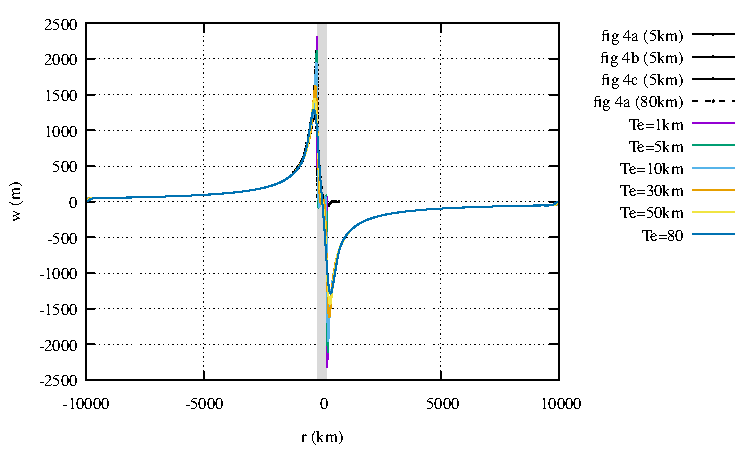
\includegraphics[width=8.4cm]{python_codes/fieldstone_108/results/w_Te.pdf}
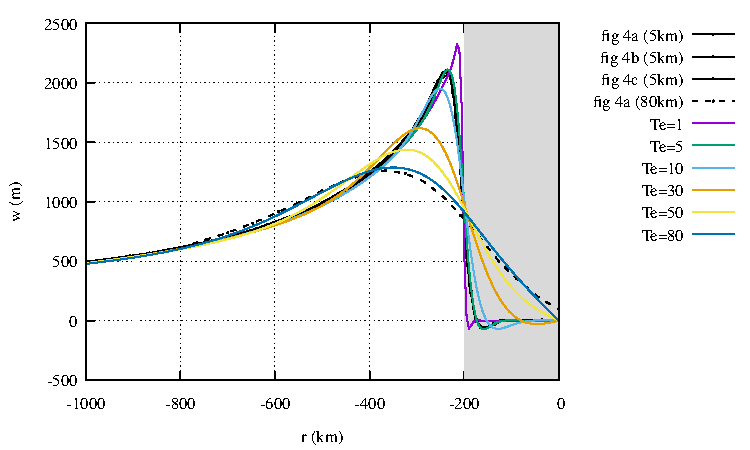
\includegraphics[width=8.4cm]{python_codes/fieldstone_108/results/w_Te_zoom.pdf}\\
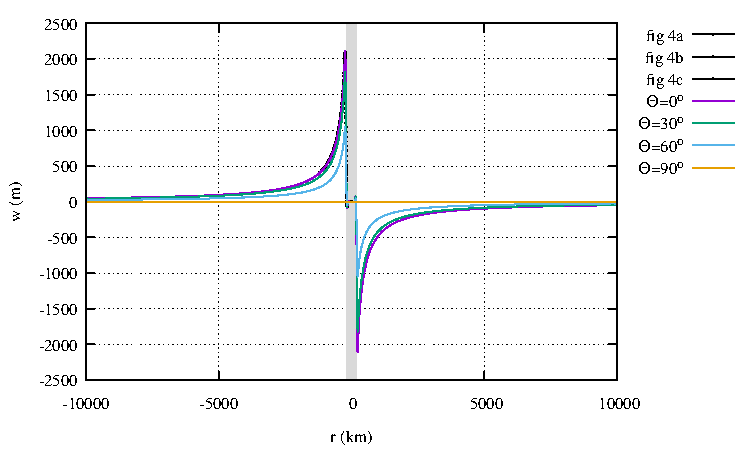
\includegraphics[width=8.4cm]{python_codes/fieldstone_108/results/w_theta.pdf}
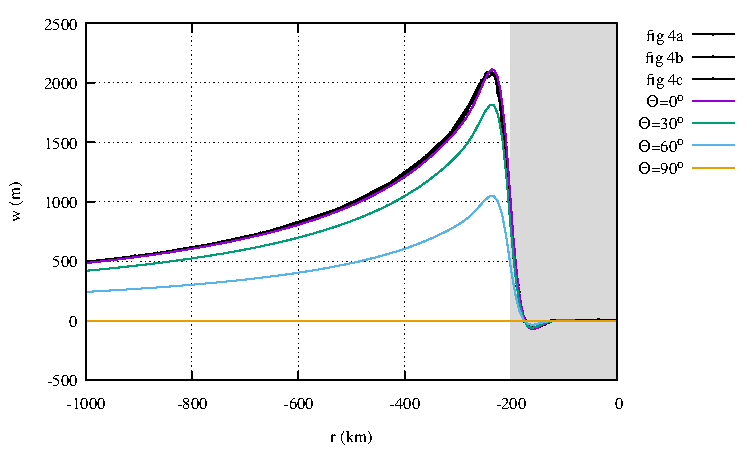
\includegraphics[width=8.4cm]{python_codes/fieldstone_108/results/w_theta_zoom.pdf}\\
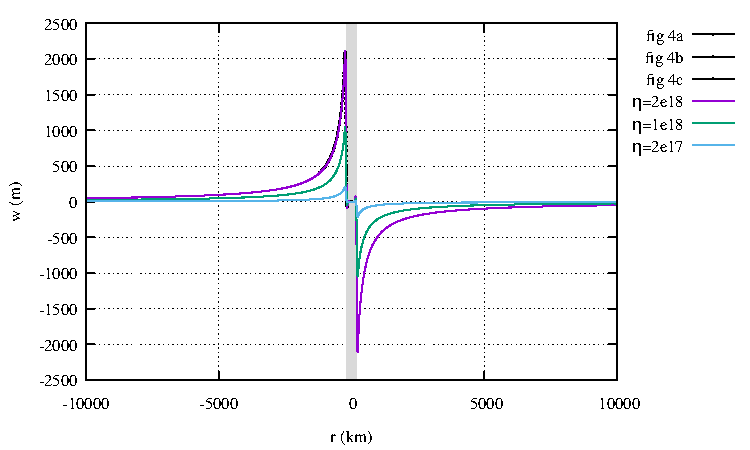
\includegraphics[width=8.4cm]{python_codes/fieldstone_108/results/w_eta.pdf}
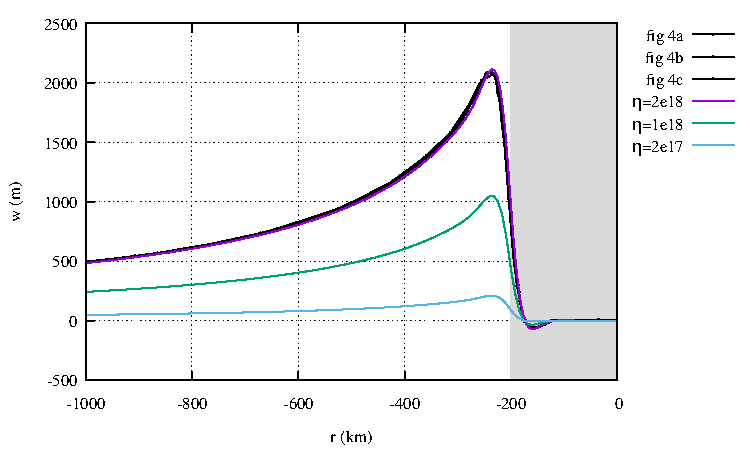
\includegraphics[width=8.4cm]{python_codes/fieldstone_108/results/w_eta_zoom.pdf}\\
{\captionfont Data from the paper were obtained with WebPlotDigitizer\footnote{\url{https://automeris.io/WebPlotDigitizer/}}. 
As mentioned above data from Fig 4b were shifted by 63km. The $r=0$ value corresponds to the center of the obstacle. The left 
column corresponds to the obtained solution over the whole domain, and the right column to the solution obtained zoomed in 
on the same range as Fig.~4 of their paper. The gray area corresponds to the obstacle.}
\end{center}

We find that we get near perfect match between our results and those of Clark \etal (2005). 


\todo[inline]{look at P again?}

\todo[inline]{prescibe pdyn only on left}
